\documentclass[conference]{IEEEtran}
\IEEEoverridecommandlockouts
% -------------------------------------------------------------------------
% CRITICAL CONFERENCE CONSTRAINT:
% MAXIMUM PAGE LIMIT: 6 PAGES (INCLUDING ALL FIGURES, TABLES, AND REFERENCES).
% DO NOT EXCEED 6 PAGES UNDER ANY CIRCUMSTANCES.
% -------------------------------------------------------------------------

\usepackage{cite}
\usepackage{amsmath,amssymb,amsfonts}
\usepackage{algorithmic}
\usepackage{graphicx}
\graphicspath{{figures/}{./}}
\usepackage{textcomp}
\usepackage{xcolor}
\usepackage{booktabs}
\usepackage{url}
\usepackage[colorlinks=true, linkcolor=blue, citecolor=blue, urlcolor=blue]{hyperref}
\setlength{\textfloatsep}{5pt plus 1pt minus 1pt}
\setlength{\floatsep}{5pt plus 1pt minus 1pt}
\setlength{\intextsep}{5pt plus 1pt minus 1pt}
\setlength{\abovecaptionskip}{3pt}
\setlength{\belowcaptionskip}{3pt}
\def\BibTeX{{\rm B\kern-.05em{\sc i\kern-.025em b}\kern-.08em
    T\kern-.1667em\lower.7ex\hbox{E}\kern-.125emX}}
\begin{document}

\title{Real-Time Driver Behavior Detection Using Lightweight Object Detection Models with Subject-Disjoint Evaluation}

\author{\IEEEauthorblockN{Oumar Mamoun Ibrahim}
\IEEEauthorblockA{\textit{Department of Computer Engineering} \\
\textit{University of Sharjah}\\
Sharjah, United Arab Emirates \\
0009-0008-0312-1605}
\and
\IEEEauthorblockN{Mohamad Khairi bin Ishak}
\IEEEauthorblockA{\textit{Department of Computer Engineering} \\
\textit{University of Sharjah}\\
Sharjah, United Arab Emirates \\
0000-0002-3554-0061}
}

\maketitle

\begin{abstract}
Driver Monitoring Systems (DMS) are critical safety components of modern Advanced Driver Assistance Systems (ADAS). While commercial systems often employ complex temporal pipelines, automotive edge deployments demand lightweight, low-latency 2D object detectors capable of real-time single-frame inference. This paper presents \textbf{DMS-Eval}, an empirical benchmark comparing compact convolutional detectors (Ultralytics YOLO11n and YOLO26n) against a lightweight Real-Time Detection Transformer (D-FINE-N). Formulated on 81 driver-facing RGB video recordings comprising 68 behavioral sessions across 14 subjects from the Driver Monitoring Dataset (DMD), the benchmark establishes 15,723 frames at $640 \times 640$. Manual Label Studio ground truth targets four visual warning cues and includes 12,722 negative frames. A frozen 8/3/3 subject-disjoint split prevents identity leakage. Shared controls include the underlying data, annotations, physical batch 8, 220-epoch ceiling, RTX 4060 target, FP16 execution policy, evaluator, and protected test procedure. The nominal effective batch is 32; backend-specific accumulation, optimization, precision, and postprocessing behavior is documented as a threat to causal architectural interpretation. Empirical result fields remain intentionally unpopulated until the frozen runs are completed.
\end{abstract}

\begin{IEEEkeywords}
driver monitoring systems, driver drowsiness detection, driver distraction detection, lightweight object detection, computer vision, YOLO, DETR, subject-disjoint evaluation, real-time edge AI
\end{IEEEkeywords}

\section{Introduction}
In-cabin Driver Monitoring Systems (DMS) constitute a vital component of modern Advanced Driver Assistance Systems (ADAS), aiming to prevent roadway collisions through early visual detection of driver drowsiness and inattention \cite{rong2021artificial,ramzan2019survey}. While high-level driver state assessment frequently leverages complex multi-frame temporal models, automotive edge deployments impose strict constraints on compute, on-chip SRAM, and per-frame latency. Consequently, there is an urgent practical demand for lightweight 2D object detectors capable of real-time single-frame inference on embedded automotive hardware.

To systematically evaluate modern compact detector paradigms under controlled single-frame constraints, this paper introduces \textbf{DMS-Eval}, an empirical benchmark comparing real-time nano-scale object detectors. We evaluate leading single-stage convolutional detectors (Ultralytics YOLO11n \cite{yolo11_ultralytics} and YOLO26n \cite{yolo26_ultralytics}) against modern end-to-end Real-Time Detection Transformers (D-FINE-N \cite{peng2024dfine}). The benchmark establishes an authoritative 15,723-frame dataset ($640\times 640$) curated from the Driver Monitoring Dataset (DMD) \cite{ortega2020dmd}, featuring 100\% manual expert ground truth across four visual warning cues (\texttt{phone\_use}, \texttt{drinking}, \texttt{yawning}, \texttt{hand\_over\_mouth}) and a naturalistic 80.91\% background negative proportion to stress false-positive suppression. To eliminate identity leakage, candidate models are evaluated on an optimal 8/3/3 subject-disjoint partition under standardized hardware and batch-1 inference profiling.

\subsection{Research Gap}
Despite substantial progress in driver monitoring, a critical methodological gap persists: \textbf{no existing study provides a reproducible, head-to-head comparison between nano-scale convolutional detectors and nano-scale Real-Time Detection Transformers for in-cabin driver cue localization under shared data, hardware, and evaluation controls with model-specific training behavior disclosed.} Existing work leaves this gap unaddressed along four axes:

\textit{(i)~Classification without spatial localization.} The AUC benchmark \cite{eraqi2019driver} and ICK-PANet \cite{qin2026ickpanet} classify full images into posture categories but produce no bounding boxes localizing the specific objects or facial cues. For edge deployment, spatial localization is essential to support downstream tracking and alert subsystems.
\textit{(ii)~Multi-stage pipelines with compounding latency.} Recent DMD studies \cite{zhang2024fatigue} chain YOLO11, AlphaPose, and LSTM networks, introducing multi-model penalties that preclude real-time edge execution. Video-sequence benchmarks \cite{Martin_2019_ICCV,ghoddoosian2019realistic} require frame buffers and recurrent state unsuitable for single-frame inference.
\textit{(iii)~Single-family evaluations.} Lightweight CNN detectors \cite{wang2024yolov10,tian2025yolov12} and real-time DETRs \cite{zhao2024detrs,peng2024dfine} are benchmarked exclusively on COCO \cite{lin2014microsoft} and never compared against each other within the in-cabin DMS domain.
\textit{(iv)~Absent evaluation rigor.} Most YOLO-based DMS studies use random frame-level splits, enabling identity leakage, and report inference speed as theoretical GFLOPs or large-batch throughput rather than the batch-size-1 latency that governs edge responsiveness \cite{reddi2020mlperf,shafi2021demystifying}.

Pinned-checkpoint smoke profiles place all three candidates below 4M parameters, motivating a resource-oriented comparison without implying that parameter storage, activations, and runtime state fit a particular microcontroller SRAM envelope. Because GFLOPs diverge from measured latency due to memory-bound attention, non-fused depthwise convolutions, and NMS overhead \cite{shafi2021demystifying}, the benchmark measures model-forward GPU latency with CUDA events at batch size~1; required postprocessing is outside this timing boundary. Final four-class parameter and FLOP values remain unreported until the trained checkpoints are profiled.

\subsection{Key Contributions}
To close the identified gap, this paper will make four contributions:
\begin{itemize}
\item \textbf{First Cross-Paradigm Nano-Scale DMS Benchmark:} The first controlled comparison between nano-scale CNNs (YOLO11n, YOLO26n) and a nano-scale DETR (D-FINE-N) for in-cabin driver cue detection with spatial bounding box localization.
\item \textbf{Rigorous Subject-Disjoint Data Curation:} 15,723 frames ($640\times640$) with 100\% manual annotation across 4 warning cues and 80.91\% naturalistic negatives, partitioned via exhaustive combinatorial optimization ($\le 5.48\%$ divergence).
\item \textbf{Unified Precision--Efficiency Protocol:} Shared RTX 4060 hardware, physical batch 8, nominal effective batch 32, 220 epochs, an FP16 execution policy, and hardware-synchronized batch-1 model-forward latency ($p50$/$p95$/$p99$), with backend-specific modes disclosed.
\item \textbf{Open Reproducibility:} Public release of all COCO annotations, partitioning scripts, and evaluation tooling.
\end{itemize}

\subsection{Research Question and Scope}
This study targets \textbf{frame-level observable cues of driver drowsiness and distraction}. Head orientation behaviors are excluded: in isolated 1~FPS frames without temporal context, safe mirror glances cannot be distinguished from dangerous inattention. The benchmark focuses on four unambiguous visual warning cues.

\begin{quote}
\textbf{RQ:} \textit{Under a shared-data, shared-hardware evaluation, how do sub-5M-parameter detectors from fundamentally different paradigms---convolutional single-stage detectors versus Real-Time Detection Transformers---compare in detection accuracy, model-forward latency, and false-alarm suppression when identifying spatial visual cues of driver distraction and drowsiness?}
\end{quote}


\section{Related Work}

\subsection{Vision-Based Driver Monitoring Systems}
Early DMS literature focused on geometric facial landmark analysis using heuristic indicators such as Eye Aspect Ratio (EAR), PERCLOS, and Mouth Aspect Ratio (MAR) \cite{ramzan2019survey}. In-cabin distraction benchmarks---including the AUC Distracted Driver dataset \cite{eraqi2019driver}, Drive\&Act \cite{Martin_2019_ICCV}, and UTA-RLDD \cite{ghoddoosian2019realistic}---advanced behavioral understanding. However, these benchmarks rely primarily on whole-frame classification or video-sequence models without spatial bounding box localization, precluding low-latency single-frame edge deployment.

\subsection{Real-Time Lightweight Object Detectors}
Convolutional detectors have evolved rapidly: YOLO11 uses C3k2 and SPPF modules \cite{yolo11_ultralytics}; YOLO26 eliminates NMS via end-to-end anchor-free design \cite{yolo26_ultralytics}; YOLOv10 introduces dual-label assignment \cite{wang2024yolov10}; and YOLOv12 incorporates attention-centric mechanisms \cite{tian2025yolov12}. In parallel, RT-DETR \cite{zhao2024detrs} adapted the DETR set-prediction paradigm \cite{carion2020detr} to real-time execution, and D-FINE \cite{peng2024dfine} refined bounding box regression via Fine-grained Distribution Refinement (FDR). However, these architectures are benchmarked on general-purpose datasets and have not been compared head-to-head within the in-cabin DMS domain.

\subsection{Subject Leakage and Evaluation Rigor}
Random train/test partitioning across identical subjects allows models to exploit driver-specific biometric features (e.g., facial morphology, clothing, seating posture) rather than generalizable behavioral semantics, artificially inflating detection accuracy \cite{rong2021artificial}. DMS-Eval strictly enforces subject-disjoint partitioning to evaluate true behavioral generalization across unseen individuals.

\section{Dataset Formulation and Annotation Protocol}

\subsection{Source Video Corpus and Spatial Standardization}
The benchmark is constructed from the Driver Monitoring Dataset (DMD) \cite{ortega2020dmd}, recorded in real vehicle cabins under variable daylight and ambient lighting conditions. The dataset encompasses 14 human subjects ($S_1\text{--}S_{14}$) across 68 distinct driving sessions, recorded as 81 driver-facing RGB video sequences ($\approx 29.76$~FPS) across three behavioral domains: \textit{distraction}, \textit{drowsiness}, and \textit{gaze}. 

To eliminate background noise outside the driver's operational workspace while preserving high spatial fidelity for fine-grained cues, every frame is uniformly sampled at 1~FPS and cropped to a standardized $640 \times 640$ pixel spatial bounding window ($x = 272, y = 71, w = 640, h = 640$) as illustrated in Fig.~\ref{fig_spatial_and_annotations}(a). This produces exactly 15,723 standardized images.

\subsection{Target Cue Ontology and Annotation Constraints}
Ground truth is generated through 100\% manual human inspection in Label Studio \cite{label_studio} with format conversion managed via \texttt{label-studio-converter} \cite{label_studio_converter}. Bounding box boundaries are defined with strict anatomical extents:
\begin{itemize}
\item \textbf{\texttt{yawning}} (ID 1): Encloses only the active mouth aperture during wide distension. Head and cheeks are excluded to prevent confusing normal open-mouth speech with yawning.
\item \textbf{\texttt{hand\_over\_mouth}} (ID 2): Encloses the full head and face including the occluding hand when placed over the mouth area.
\item \textbf{\texttt{drinking}} (ID 3): Encloses the interacting hand and the beverage container together during active consumption posture.
\item \textbf{\texttt{phone\_use}} (ID 4): Encloses the handheld device and interacting hand held to the ear/head in calling posture.
\end{itemize}

\begin{figure}[htbp]
\centering

\includegraphics[width=0.92\columnwidth]{640X640.png}\\[3pt]
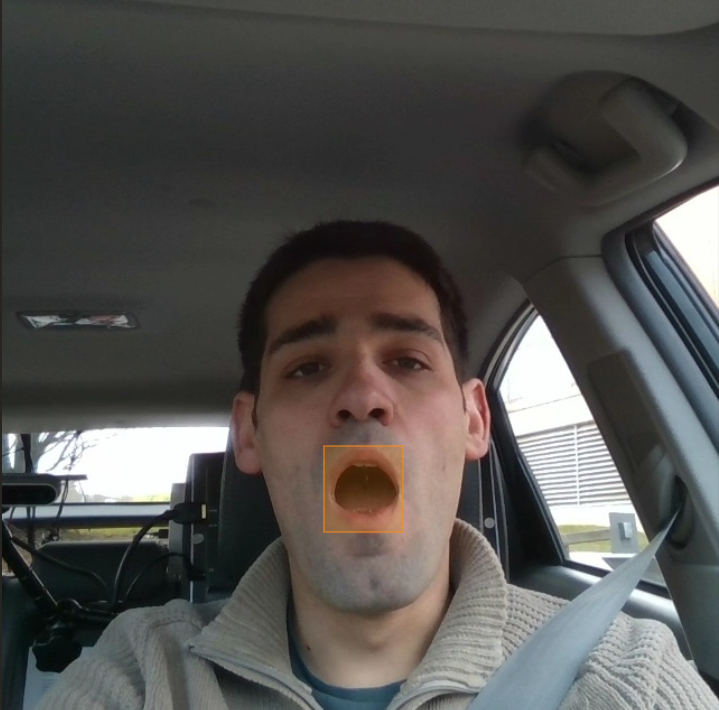
\includegraphics[width=0.46\columnwidth]{yawning_annotation_example.png}\hfill
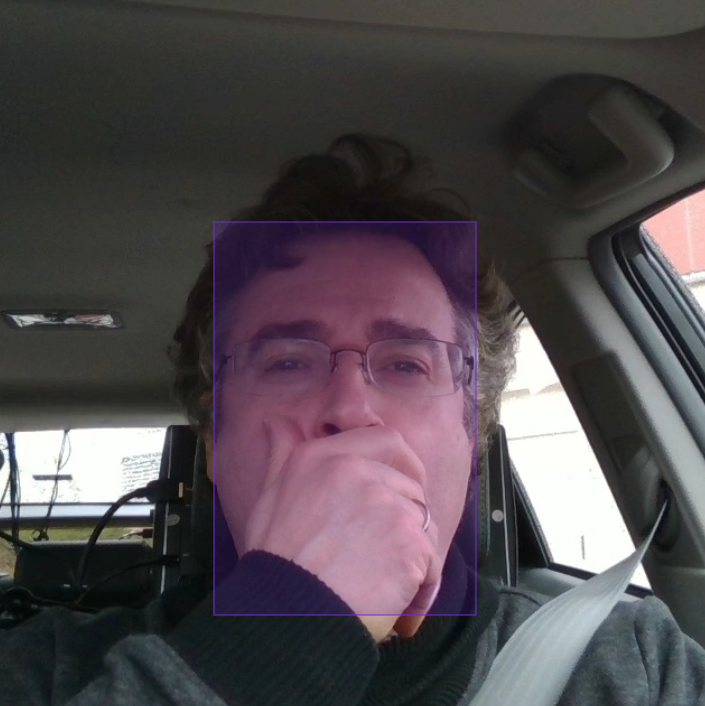
\includegraphics[width=0.46\columnwidth]{hand_over_mouth_annotation_example.png}\\[2pt]
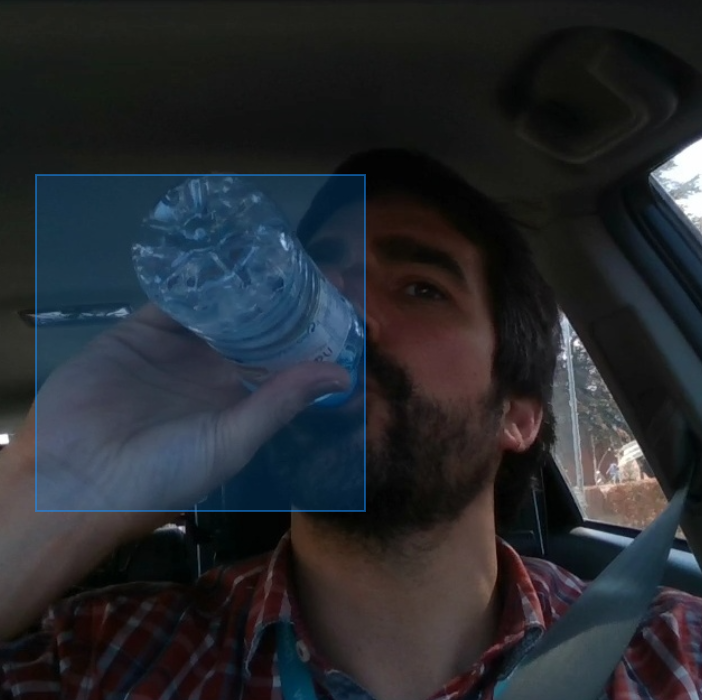
\includegraphics[width=0.46\columnwidth]{drinking_annotation_example.png}\hfill
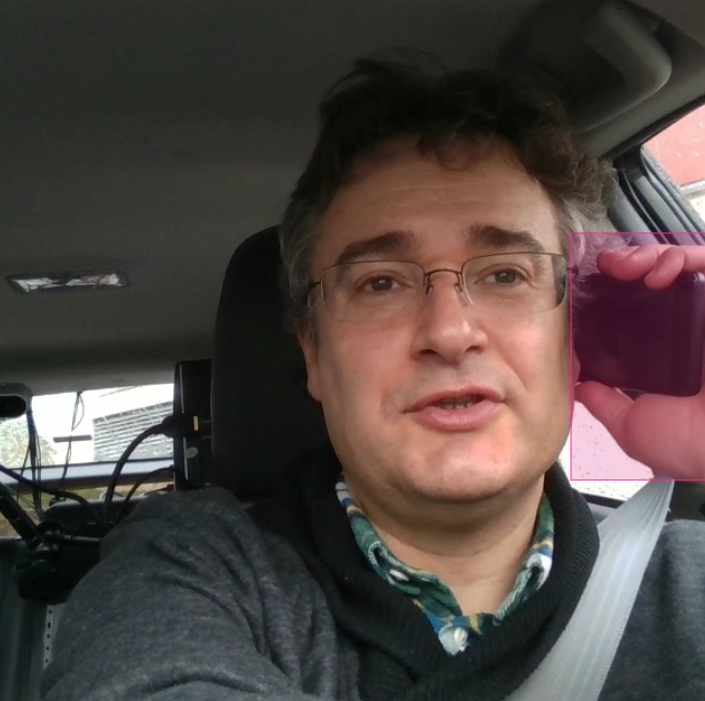
\includegraphics[width=0.46\columnwidth]{phone_use_annotation_example.png}
\caption{DMS-Eval spatial cropping and ground-truth warning cue annotations: (a) standardized $640 \times 640$ spatial window crop ($x=272, y=71$) centering the driver workspace; (b) \texttt{yawning} (mouth aperture only); (c) \texttt{hand\_over\_mouth} (full head enclosing occluding hand); (d) \texttt{drinking} (hand and container in active consumption); (e) \texttt{phone\_use} (handheld device at ear in calling posture).}
\label{fig_spatial_and_annotations}
\end{figure}

\subsection{Single-Annotation and Mutual Exclusivity Protocol}
Under our single-frame protocol, each sampled frame contains at most one bounding box ($0$ or $1$ box). In particular, \texttt{yawning} and \texttt{hand\_over\_mouth} are strictly mutually exclusive. If a driver yawns while a hand visibly occludes the mouth, the frame is uniquely labeled as \texttt{hand\_over\_mouth}. This eliminates ambiguous overlapping bounding boxes and ensures sharp ground-truth targets.

\subsection{Negative Sample Richness}
By incorporating all three DMD session folders, our benchmark contains 12,722 true negative background frames ($80.91\%$) and 3,001 positive cue frames ($19.09\%$) as shown in Fig.~\ref{fig_distributions_and_splits}(a)--(b).

\section{Methodology and Subject-Disjoint Partitioning}

\subsection{Subject-Disjoint Splitting Principle}
To eliminate identity leakage, the 14 subjects are partitioned into 8 Training, 3 Validation, and 3 Test subjects such that:
\begin{equation}
S_{\text{train}} \cap S_{\text{val}} = \emptyset, \quad S_{\text{train}} \cap S_{\text{test}} = \emptyset, \quad S_{\text{val}} \cap S_{\text{test}} = \emptyset
\end{equation}

\subsection{Exhaustive Proportion-Matching Optimization}
Because subjects naturally exhibit varying behavioral frequencies, random assignment often results in severe class imbalance. We formalize an authoritative selection rule:
\begin{quote}
\textit{Select the 8/3/3 subject split whose negative/positive frame proportion and four class proportions most closely match the complete dataset distribution.}
\end{quote}

Our algorithm evaluates all $\binom{14}{8}\binom{6}{3}=60{,}060$ ordered 8/3/3 subject assignments. For each candidate partition $\mathcal{P}\in\Omega$ and split $s\in\{\mathrm{train,val,test}\}$, we compute absolute relative deviation for positive-frame rate and each of the four named cue proportions:
\begin{equation}
\text{Dev}(q, s) = \frac{\vert V(q, s) - V_{\text{global}}(q) \vert}{V_{\text{global}}(q)}
\end{equation}
Candidate partitions are ranked via a deterministic lexicographic objective:
\begin{equation}
\mathcal{P}^* = \arg\min_{\mathcal{P} \in \Omega} \left( \max_{q \in \mathcal{Q}, s \in \mathcal{S}} \text{Dev}(q, s), \, \text{RMSE}(\mathcal{P}), \, \text{Dev}_{\text{test}}(\mathcal{P}) \right)
\end{equation}

\subsection{Frozen Split Statistics}
The optimal partition selected by the algorithm is permanently frozen in \texttt{dataset/splits.json}:
\begin{itemize}
\item \textbf{Train} (8 subjects): $S_1, S_4, S_6, S_7, S_8, S_9, S_{13}, S_{14}$
\item \textbf{Validation} (3 subjects): $S_2, S_3, S_{11}$
\item \textbf{Test} (3 subjects): $S_5, S_{10}, S_{12}$
\end{itemize}

As documented in Table~\ref{tab_splits} and Fig.~\ref{fig_distributions_and_splits}(c), the maximum relative deviation across all splits and classes is restricted to $\le 5.4812\%$, yielding closely matched distributions across partitions.

\begin{figure}[htbp]
\centering
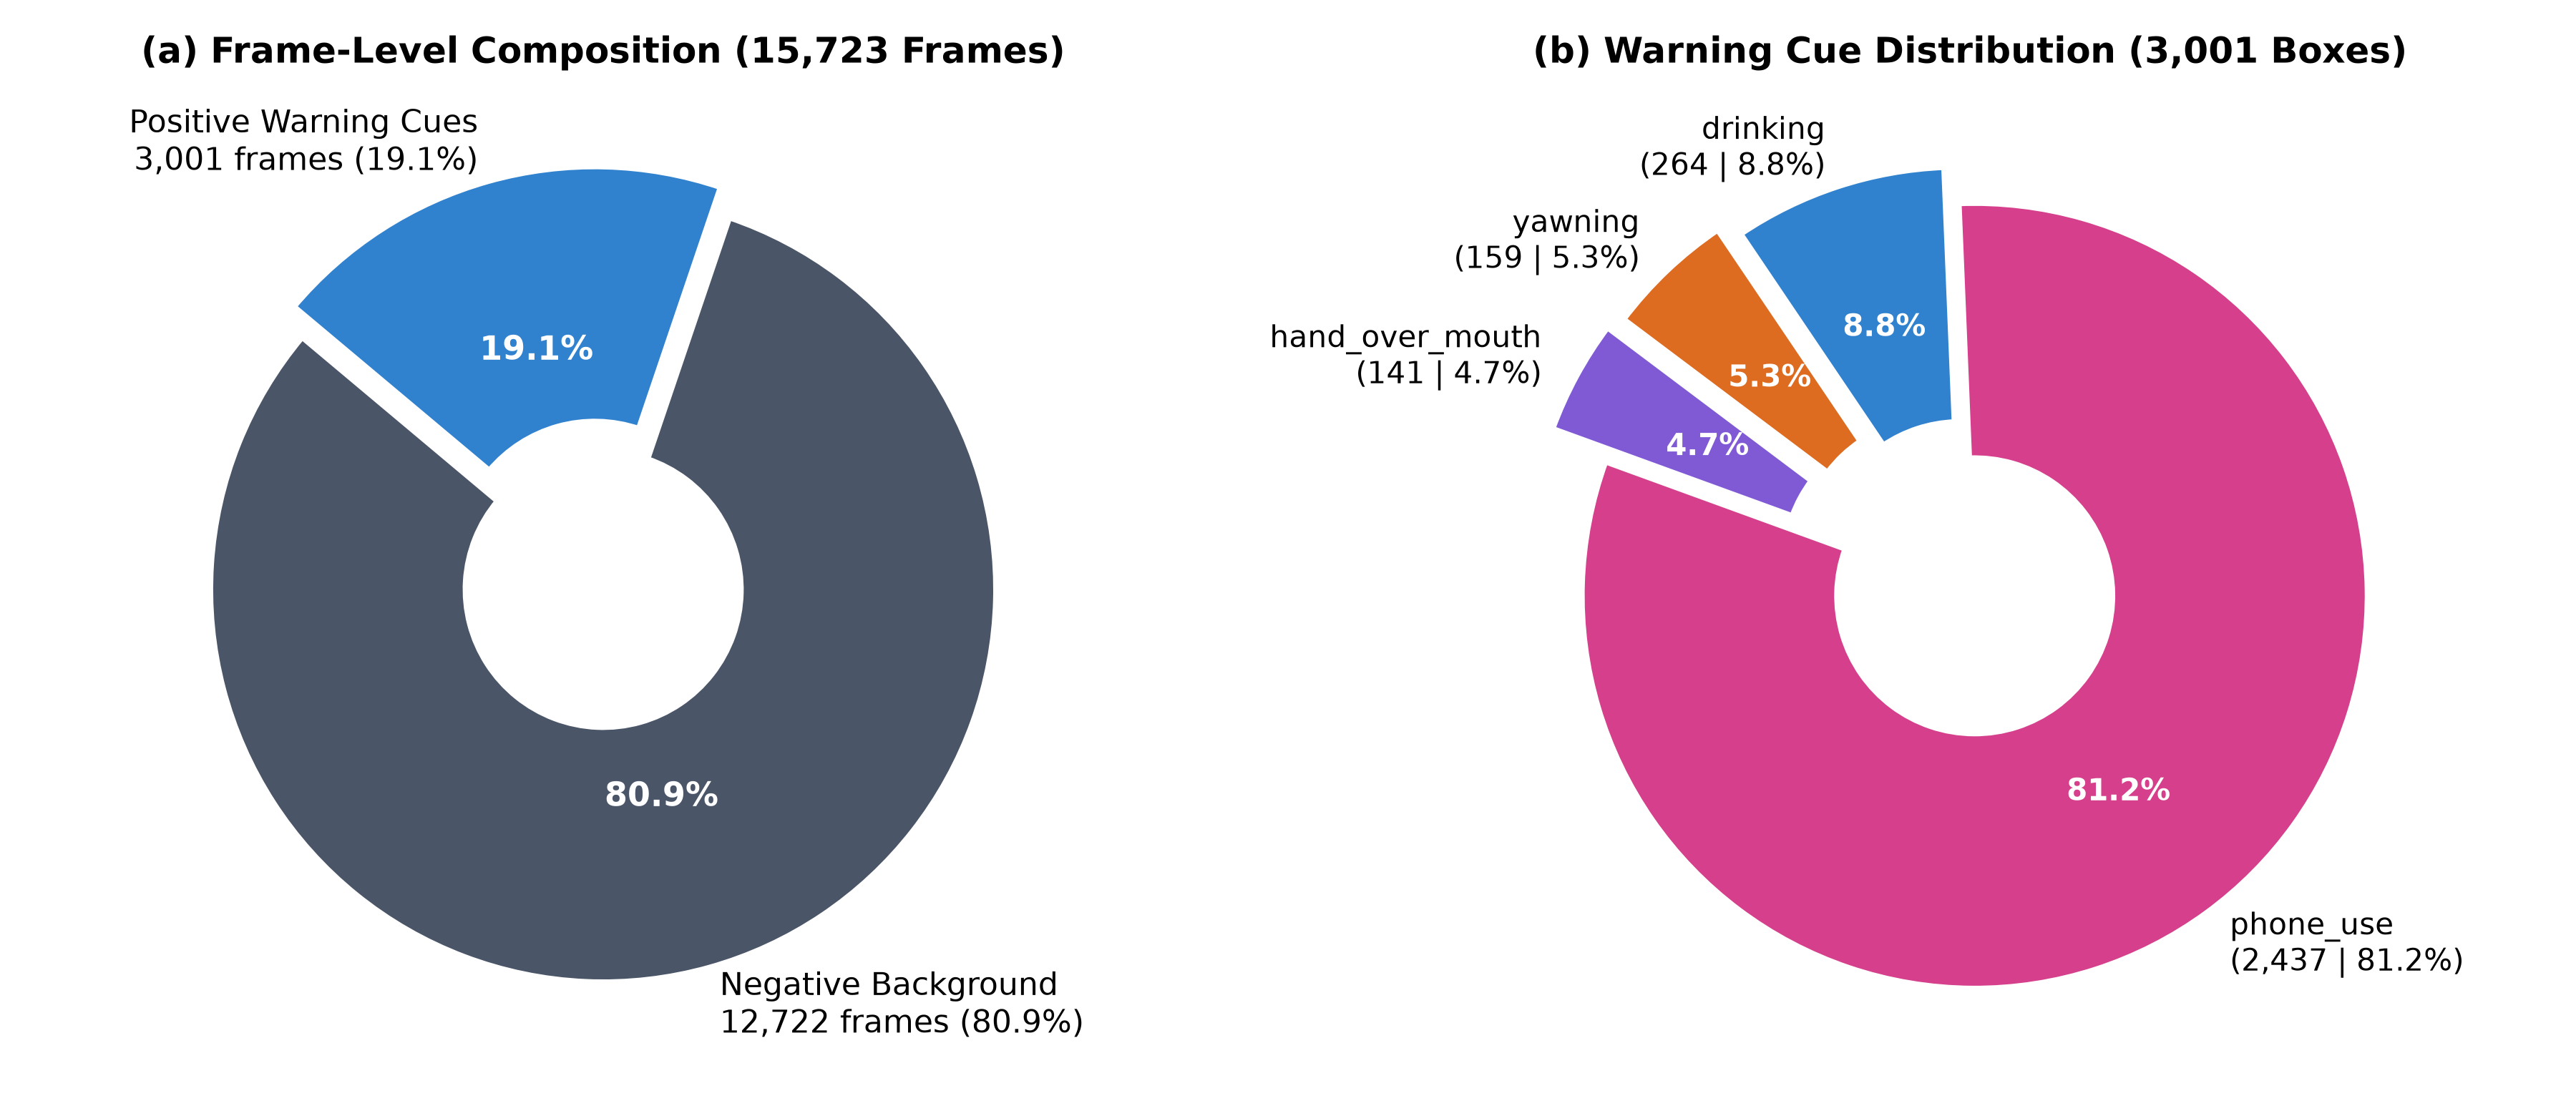
\includegraphics[width=0.92\columnwidth]{benchmark_distributions_combined.png}\\[3pt]

\includegraphics[width=0.92\columnwidth]{split_cue_proportions_comparison.png}
\caption{DMS-Eval dataset composition and split fidelity: (a) frame-level composition ($80.91\%$ negative background frames); (b) target cue proportions across 3,001 bounding boxes; (c) warning cue distribution preservation across 8/3/3 subject-disjoint partitions ($\le 5.4812\%$ maximum relative divergence).}
\label{fig_distributions_and_splits}
\end{figure}

\subsection{Temporal Shuffling and Sequence Preservation}
Because 1~FPS extraction from continuous driving video introduces temporal correlation between adjacent frames, a deterministic pseudo-random permutation (seed 13) is applied exclusively to the training split ($S_{\text{train}}$) to diversify mini-batch gradient updates and prevent sequential overfitting. Conversely, validation and test splits ($S_{\text{val}}, S_{\text{test}}$) are strictly preserved in their native chronological order to enable contiguous temporal error analysis and ensure benchmark compatibility with future sequence-based architectures.

\begin{table}[htbp]
\caption{Dataset Split Composition and Warning Cue Distributions Across Partitions}
\begin{center}
\resizebox{\columnwidth}{!}{
\begin{tabular}{lrrrrrrrr}
\toprule
\textbf{Split} & \textbf{Total} & \textbf{Negatives} & \textbf{Positives} & \textbf{Pos. Rate} & \textbf{\texttt{phone\_use}} & \textbf{\texttt{drinking}} & \textbf{\texttt{yawning}} & \textbf{\texttt{hand\_over\_mouth}} \\
\midrule
\textbf{Global} & \textbf{15,723} & \textbf{12,722} & \textbf{3,001} & \textbf{19.09\%} & \textbf{2,437 (81.2\%)} & \textbf{264 (8.8\%)} & \textbf{159 (5.3\%)} & \textbf{141 (4.7\%)} \\
\textbf{Train}  & 9,087  & 7,339  & 1,748 & 19.24\% & 1,417 (81.1\%) & 154 (8.8\%) & 94 (5.4\%)  & 83 (4.7\%) \\
\textbf{Val}    & 3,423  & 2,784  & 639   & 18.67\% & 523 (81.9\%)   & 54 (8.5\%)  & 32 (5.0\%)  & 30 (4.7\%) \\
\textbf{Test}   & 3,213  & 2,599  & 614   & 19.11\% & 497 (80.9\%)   & 56 (9.1\%)  & 33 (5.4\%)  & 28 (4.6\%) \\
\bottomrule
\end{tabular}
}
\label{tab_splits}
\end{center}
\end{table}

\begin{figure*}[htbp]
\centerline{
\includegraphics[width=\textwidth]{dms_eval_pipeline.png}}
\caption{DMS-Eval benchmark lifecycle: standardized $640\times 640$ extraction from 81 DMD videos; Label Studio ground truth across 4 warning cues (80.91\% negative frames); deterministic 8/3/3 subject-disjoint splitting ($\le 5.48\%$ relative divergence); RTX 4060 training with physical batch 8, nominal batch 32, 220 epochs, seed 13, and disclosed backend-specific accumulation; validation-only $F_1$ threshold calibration ($\tau^*$); and isolated single-pass test evaluation.}
\label{fig_pipeline}
\end{figure*}

\section{Experimental Setup and Evaluation Protocol}
The overall end-to-end benchmark methodology, spanning dataset ingestion, subject-disjoint partitioning, training controls, validation calibration, and isolated test evaluation, is illustrated in Fig.~\ref{fig_pipeline}.

\subsection{Evaluated Model Architectures}
We evaluate three state-of-the-art nano-scale real-time object detectors:
\begin{enumerate}
\item \textbf{Ultralytics YOLO11n} \cite{yolo11_ultralytics}: Compact convolutional single-stage detector featuring C3k2 and SPPF modules. Its loss optimizes Complete IoU (CIoU), Binary Cross-Entropy (BCE), and Distribution Focal Loss (DFL):
\begin{equation}
\mathcal{L}_{\text{YOLO11}} = \lambda_{\text{box}}\mathcal{L}_{\text{CIoU}} + \lambda_{\text{cls}}\mathcal{L}_{\text{BCE}} + \lambda_{\text{dfl}}\mathcal{L}_{\text{DFL}}
\end{equation}
\item \textbf{Ultralytics YOLO26n} \cite{yolo26_ultralytics}: NMS-free end-to-end detector using dual-label one-to-one assignment.
\item \textbf{D-FINE-N} \cite{peng2024dfine}: Lightweight Real-Time Detection Transformer with an HGNetv2 backbone and Fine-grained Distribution Refinement, optimized via Hungarian set loss:
\begin{equation}
\mathcal{L}_{\text{D-FINE}} = \lambda_{\text{cls}}\mathcal{L}_{\text{VFL}} + \lambda_{\text{box}}\mathcal{L}_{\text{GIoU}} + \lambda_{\text{fdr}}\mathcal{L}_{\text{FDR}} + \mathcal{L}_{\text{GO-LSD}}
\end{equation}
\end{enumerate}

\subsection{Standardized Training Protocol}
All models are fine-tuned under the following shared controls:
\begin{itemize}
\item \textbf{Fine-Tuning Budget}: Exactly 220 epochs without early stopping.
\item \textbf{Batch Size \& Gradient Dynamics}: Physical mini-batch size is locked to 8 with nominal effective batch 32. D-FINE uses fixed four-step accumulation; Ultralytics \texttt{nbs=32} ramps accumulation from 1 toward 4 during warm-up before settling at 4.
\item \textbf{Random Seed}: Seed 13 is passed to each framework without claiming identical sampler order or stochastic trajectories across implementations.
\item \textbf{Precision}: FP16 Automatic Mixed Precision (AMP).
\item \textbf{Hardware Platform}: Dedicated NVIDIA GeForce RTX 4060 GPU (8~GB VRAM).
\end{itemize}

Optimization hyperparameters are benchmark-pinned and model specific: the YOLO launchers use SGD with momentum 0.937, whereas D-FINE uses AdamW with a base learning rate of 0.00025 and backbone learning rate of 0.0000125. These values are explicit reproducibility choices rather than unchanged reproductions of every pinned upstream default. Additional backend behavior remains unequal: D-FINE drops incomplete training batches and its two-stage solver reloads the best stage-1 validation checkpoint at epoch 148, whereas YOLO retains incomplete batches and follows a continuous trajectory. Final reported checkpoints for all models are nevertheless ranked by the same shared validation $\text{mAP}@0.5:0.95$ procedure. These distinctions prevent interpreting the comparison as an isolation of architecture alone.

\subsection{Validation Calibration and Test Isolation}
To prevent data snooping, model checkpoints and confidence thresholds ($\tau$) are selected strictly on the Validation split. For each model, we sweep confidence thresholds $\tau \in [0.01, 0.99]$ with a step of $0.01$ and identify the threshold $\tau^*$ that maximizes the micro-averaged $F_1$ score:
\begin{equation}
\tau^* = \arg\max_{\tau \in [0.01, 0.99]} F_1(\tau; S_{\text{val}}) = \frac{2 \cdot P(\tau) \cdot R(\tau)}{P(\tau) + R(\tau)}
\end{equation}
where $P(\tau) = \frac{\text{TP}(\tau)}{\text{TP}(\tau) + \text{FP}(\tau)}$ and $R(\tau) = \frac{\text{TP}(\tau)}{\text{TP}(\tau) + \text{FN}(\tau)}$ under same-class greedy one-to-one IoU $\ge 0.50$ matching. The optimal validation checkpoint and threshold $\tau^*$ are permanently frozen. Final benchmark evaluation is executed in a single pass on the unseen Test split ($S_{\text{test}}$) without further tuning.

\subsection{Latency, Memory, and False-Alarm Profiling}
Inference profiling uses native PyTorch on the RTX 4060 at batch size 1 under an FP16 execution policy. YOLO uses FP16 weights and input, whereas D-FINE uses an FP16 input under CUDA autocast; operator-level precision is therefore not identical. Following 10 untimed warm-up passes, model-forward GPU latency is measured across all test frames using synchronized CUDA events (\texttt{torch.cuda.Event}). Disk I/O, decoding, preprocessing, postprocessing/NMS, and metrics are excluded, so the reported latency is not end-to-end deployment latency. We report $p50$, $p95$, $p99$, and sustained model-forward FPS, and measure peak allocation using \texttt{torch.cuda.max\_memory\_allocated()}. False-alarm suppression is evaluated on the 2,599 negative frames in the protected test split:
\begin{equation}
\text{FAR}_{100} = \frac{\text{FP detections on negative frames}}{2{,}599} \times 100
\end{equation}
and is interpreted as false detections per 100 negative test frames rather than a percentage bounded by 100.

\section{Benchmark Results Framework}
The controlled comparative evaluation results across detection accuracy, hardware runtime efficiency, peak memory allocation, and false-alarm suppression on the unseen test split ($S_{\text{test}}$) are reported in Table~\ref{tab_results}. Table~\ref{tab_per_class} details the fine-grained per-class Average Precision breakdown across the four target warning cues.

\begin{table*}[htbp]
\caption{Comparative Evaluation Framework (RTX 4060, Batch Size 1, FP16 Policy, Model-Forward Timing)}
\begin{center}
\resizebox{\textwidth}{!}{
\begin{tabular}{lccccccccccccr}
\toprule
\textbf{Model} & \textbf{Params} & \textbf{FLOPs} & \textbf{VRAM (MB)} & \textbf{Lat. $p50$} & \textbf{Lat. $p95$} & \textbf{Lat. $p99$} & \textbf{FPS} & \textbf{FAR$_{100}$} & \textbf{mAP@0.5:0.95} & \textbf{mAP@0.5} & \textbf{Prec.} & \textbf{Recall} & \textbf{F1} \\
\midrule
YOLO11n & Not run & Not run & Not run & Not run & Not run & Not run & Not run & Not run & Not run & Not run & Not run & Not run & Not run \\
YOLO26n & Not run & Not run & Not run & Not run & Not run & Not run & Not run & Not run & Not run & Not run & Not run & Not run & Not run \\
D-FINE-N & Not run & Not run & Not run & Not run & Not run & Not run & Not run & Not run & Not run & Not run & Not run & Not run & Not run \\
\bottomrule
\end{tabular}
}
\label{tab_results}
\end{center}
\end{table*}

\begin{table}[htbp]
\caption{Per-Class Detection Performance Framework ($mAP@0.5:0.95$ / $mAP@0.5$ on Test Split)}
\begin{center}
\resizebox{\columnwidth}{!}{
\begin{tabular}{lcccc}
\toprule
\textbf{Model} & \textbf{\texttt{phone\_use}} & \textbf{\texttt{drinking}} & \textbf{\texttt{yawning}} & \textbf{\texttt{hand\_over\_mouth}} \\
\midrule
YOLO11n & Not run & Not run & Not run & Not run \\
YOLO26n & Not run & Not run & Not run & Not run \\
D-FINE-N & Not run & Not run & Not run & Not run \\
\bottomrule
\end{tabular}
}
\label{tab_per_class}
\end{center}
\end{table}

\section{Discussion, Failure Analysis, and Threats to Validity}

\subsection{Architectural Trade-offs at Edge Scale}
The planned evaluation is designed to expose trade-offs between inductive bias and global receptive field. Convolutional backbones (YOLO11n, YOLO26n) provide strong spatial locality, whereas D-FINE-N uses cross-scale attention; the measured benchmark will determine how those properties trade accuracy against latency and memory on the frozen hardware. No comparative empirical conclusion is asserted before the protected test pass.

\subsection{Taxonomy of Edge-Case Failure Modes}
The post-test error analysis is pre-registered around three anticipated edge-case categories:
\begin{itemize}
\item \textbf{High-Frequency Motion Blur:} Test whether rapid gestures and steering transitions correspond to missed detections or localization jitter.
\item \textbf{Extreme Ambient Illumination Transitions:} Test whether glare and cabin shadows correspond to false-positive facial-cue detections.
\item \textbf{Oblique Head Yaw and Occlusion:} Test whether lateral head turns and partial occlusion challenge single-frame localization.
\end{itemize}

\subsection{Threats to Validity}
\begin{itemize}
\item \textbf{Internal Validity:} Shared data, validation-only selection, and protected testing limit leakage, but do not isolate architecture. YOLO accumulation ramps; D-FINE uses fixed accumulation, drops incomplete batches, and reloads its best stage-1 checkpoint. Recipes lack a common tuning budget, and one seed does not quantify run variance.
\item \textbf{Runtime Construct Validity:} Timings cover model forward only, excluding postprocessing/NMS. YOLO uses FP16 weights while D-FINE uses autocast, and raw checkpoints contain different payloads; latency and file size are not standardized end-to-end deployment measures.
\item \textbf{External Validity:} Performance may vary under extreme nighttime illumination or across unobserved camera mounting angles.
\end{itemize}

\section{Conclusion}
This paper introduces \textbf{DMS-Eval}, a reproducible benchmark for lightweight in-cabin detectors. Its 15,723-frame dataset, four warning cues, subject-disjoint split, shared evaluator, and protected test procedure address key leakage risks. The frozen runs will compare three configured systems under declared controls; architecture-only claims remain bounded by the documented recipe, precision, postprocessing, serialization, and single-run limitations.

\section*{Acknowledgment}
We acknowledge the open-source Ultralytics YOLO \cite{yolo11_ultralytics,yolo26_ultralytics}, D-FINE \cite{peng2024dfine}, and Label Studio \cite{label_studio,label_studio_converter} projects.

% must not exceed the 6-page maximum limit.
% -------------------------------------------------------------------------

\begin{thebibliography}{00}
\setlength{\itemsep}{1pt plus 0.5pt minus 0.5pt}

\bibitem{yolo11_ultralytics}
G.~Jocher and J.~Qiu, ``Ultralytics {YOLO11},'' 2024. [Online]. Available: \url{https://github.com/ultralytics/ultralytics}

\bibitem{yolo26_ultralytics}
G.~Jocher, J.~Qiu, and A.~Chaurasia, ``Ultralytics {YOLO26}: End-to-End Real-Time Object Detection,'' 2026. [Online]. Available: \url{https://github.com/ultralytics/ultralytics}

\bibitem{peng2024dfine}
Y.~Peng, H.~Li, P.~Wu, Y.~Zhang, X.~Sun, and F.~Wu, ``{D-FINE}: Redefining Bounding Box Regression for End-to-End Real-Time Object Detection,'' \textit{arXiv preprint arXiv:2410.13842}, 2024.

\bibitem{zhao2024detrs}
Y.~Zhao, W.~Lv, S.~Xu, J.~Wei, G.~Wang, Q.~Dang, Y.~Liu, and J.~Chen, ``{DETRs} Beat {YOLOs} on Real-Time Object Detection,'' in \textit{Proc. IEEE/CVF Conf. Comput. Vis. Pattern Recognit. (CVPR)}, 2024, pp. 16965--16974.

\bibitem{carion2020detr}
N.~Carion, F.~Massa, G.~Synnaeve, N.~Usunier, A.~Kirillov, and S.~Zagoruyko, ``End-to-End Object Detection with Transformers,'' in \textit{Computer Vision -- ECCV 2020}, Springer, 2020, pp. 213--229.

\bibitem{wang2024yolov10}
A.~Wang, H.~Chen, L.~Liu, K.~Chen, Z.~Lin, J.~Han, and G.~Ding, ``{YOLOv10}: Real-Time End-to-End Object Detection,'' in \textit{Adv. Neural Inf. Process. Syst. (NeurIPS)}, 2024.

\bibitem{tian2025yolov12}
Y.~Tian, Q.~Ye, \textit{et al.}, ``{YOLOv12}: Attention-Centric Real-Time Object Detectors,'' \textit{arXiv preprint arXiv:2502.12524}, 2025.

\bibitem{ortega2020dmd}
J.~D. Ortega, N.~Kose, P.~Ca{\~n}as, M.-A. Chao, A.~Unnervik, M.~Nieto, O.~Otaegui, and L.~Salgado, ``{DMD}: A Large-Scale Multi-Modal Driver Monitoring Dataset for Attention and Alertness Analysis,'' in \textit{Computer Vision -- ECCV 2020 Workshops}, Springer, 2020, pp. 387--405.

\bibitem{eraqi2019driver}
H.~M. Eraqi, Y.~Abouelnaga, M.~H. Saad, and M.~N. Moustafa, ``Driver Distraction Identification with an Ensemble of Convolutional Neural Networks,'' \textit{J. Adv. Transp.}, vol. 2019, pp. 1--12, 2019.

\bibitem{Martin_2019_ICCV}
M.~Martin, A.~Roitberg, M.~Haurilet, M.~Horne, C.~Rei{\ss}, M.~Voit, and R.~Stiefelhagen, ``{Drive\&Act}: A Multi-Modal Dataset for Fine-Grained Driver Behavior Recognition in Autonomous Vehicles,'' in \textit{Proc. IEEE/CVF Int. Conf. Comput. Vis. (ICCV)}, 2019, pp. 2801--2810.

\bibitem{lin2014microsoft}
T.-Y. Lin, M.~Maire, S.~Belongie, J.~Hays, P.~Perona, D.~Ramanan, P.~Doll{\'a}r, and C.~L. Zitnick, ``Microsoft {COCO}: Common Objects in Context,'' in \textit{Computer Vision -- ECCV 2014}, Springer, 2014, pp. 740--755.

\bibitem{ghoddoosian2019realistic}
R.~Ghoddoosian, M.~Galib, and V.~Athitsos, ``A Realistic Dataset and Baseline Temporal Model for Detecting Driver Drowsiness in the Wild,'' in \textit{Proc. IEEE/CVF Conf. Comput. Vis. Pattern Recognit. (CVPR) Workshops}, 2019, pp. 1--10.

\bibitem{qin2026ickpanet}
B.~Qin, B.~Zhang, and J.~Qian, ``{ICK-PANet}: A Multiscale Driver Distraction Detection Network Based on Attention and Pyramid Convolution,'' \textit{Vehicles}, vol. 8, no. 4, p. 83, 2026.

\bibitem{zhang2024fatigue}
Y.~Zhang, X.~Wang, and Z.~Sheng, ``Multi-View Driver Fatigue Detection Based on Optimized {YOLO11} and {AlphaPose},'' \textit{Sensors}, vol. 24, no. 18, p. 5912, 2024.

\bibitem{reddi2020mlperf}
V.~J. Reddi \textit{et al.}, ``{MLPerf} Inference Benchmark,'' \textit{IEEE Micro}, vol. 40, no. 3, pp. 8--16, 2020.

\bibitem{shafi2021demystifying}
O.~Shafi \textit{et al.}, ``Demystifying {TensorRT}: An In-Depth Analysis to Accelerate Deep Learning Inference on Edge {GPUs},'' \textit{IEEE Access}, vol. 9, pp. 102435--102450, 2021.

\bibitem{rong2021artificial}
Y.~Rong \textit{et al.}, ``In-Cabin Driver Monitoring Systems: A Survey on Vision-Based Approaches,'' \textit{IEEE Trans. Intell. Veh.}, vol. 6, no. 4, pp. 728--748, 2021.

\bibitem{ramzan2019survey}
M.~Ramzan \textit{et al.}, ``A Survey on State-of-the-Art Drowsiness Detection Techniques,'' \textit{IEEE Access}, vol. 7, pp. 61904--61919, 2019.

\bibitem{label_studio}
HumanSignal, ``Label Studio: Open Source Data Labeling Tool,'' 2024. [Online]. Available: \url{https://github.com/HumanSignal/label-studio}

\bibitem{label_studio_converter}
HumanSignal, ``Label Studio Converter: Format Exporters and Converters for Label Studio Annotations,'' 2024. [Online]. Available: \url{https://github.com/HumanSignal/label-studio-converter}

\end{thebibliography}

% -------------------------------------------------------------------------
% REMINDER: Ensure paper does not exceed the 6-page maximum limit.
% -------------------------------------------------------------------------

\end{document}
